\subsection{6g Tri-Axial Accelerometer Data}

The MMA7361LC accelerometer was deployed in the computer room on the north side of the east tower, 40 feet from the top of the tower. The package collected four 60 second samples, all at 100 Hz. The package was mounted such that x is vertical, y aligned with the length of the bridge, and z is the lateral axis

\indent The Fourier transform of each axis of each sample was taken to identify resonant frequencies . The first and fourth data set show a broadband frequency below 0.4 Hz in the Y axis, seen in figure \ref{fig:fftall}.

\indent Peak accelerations did not exceed 0.1 $m/s^2$. Using the accelerometer’s 1.5 g setting would be more appropriate for this application, yielding a higher resolution. 

\begin{figure}
\centering
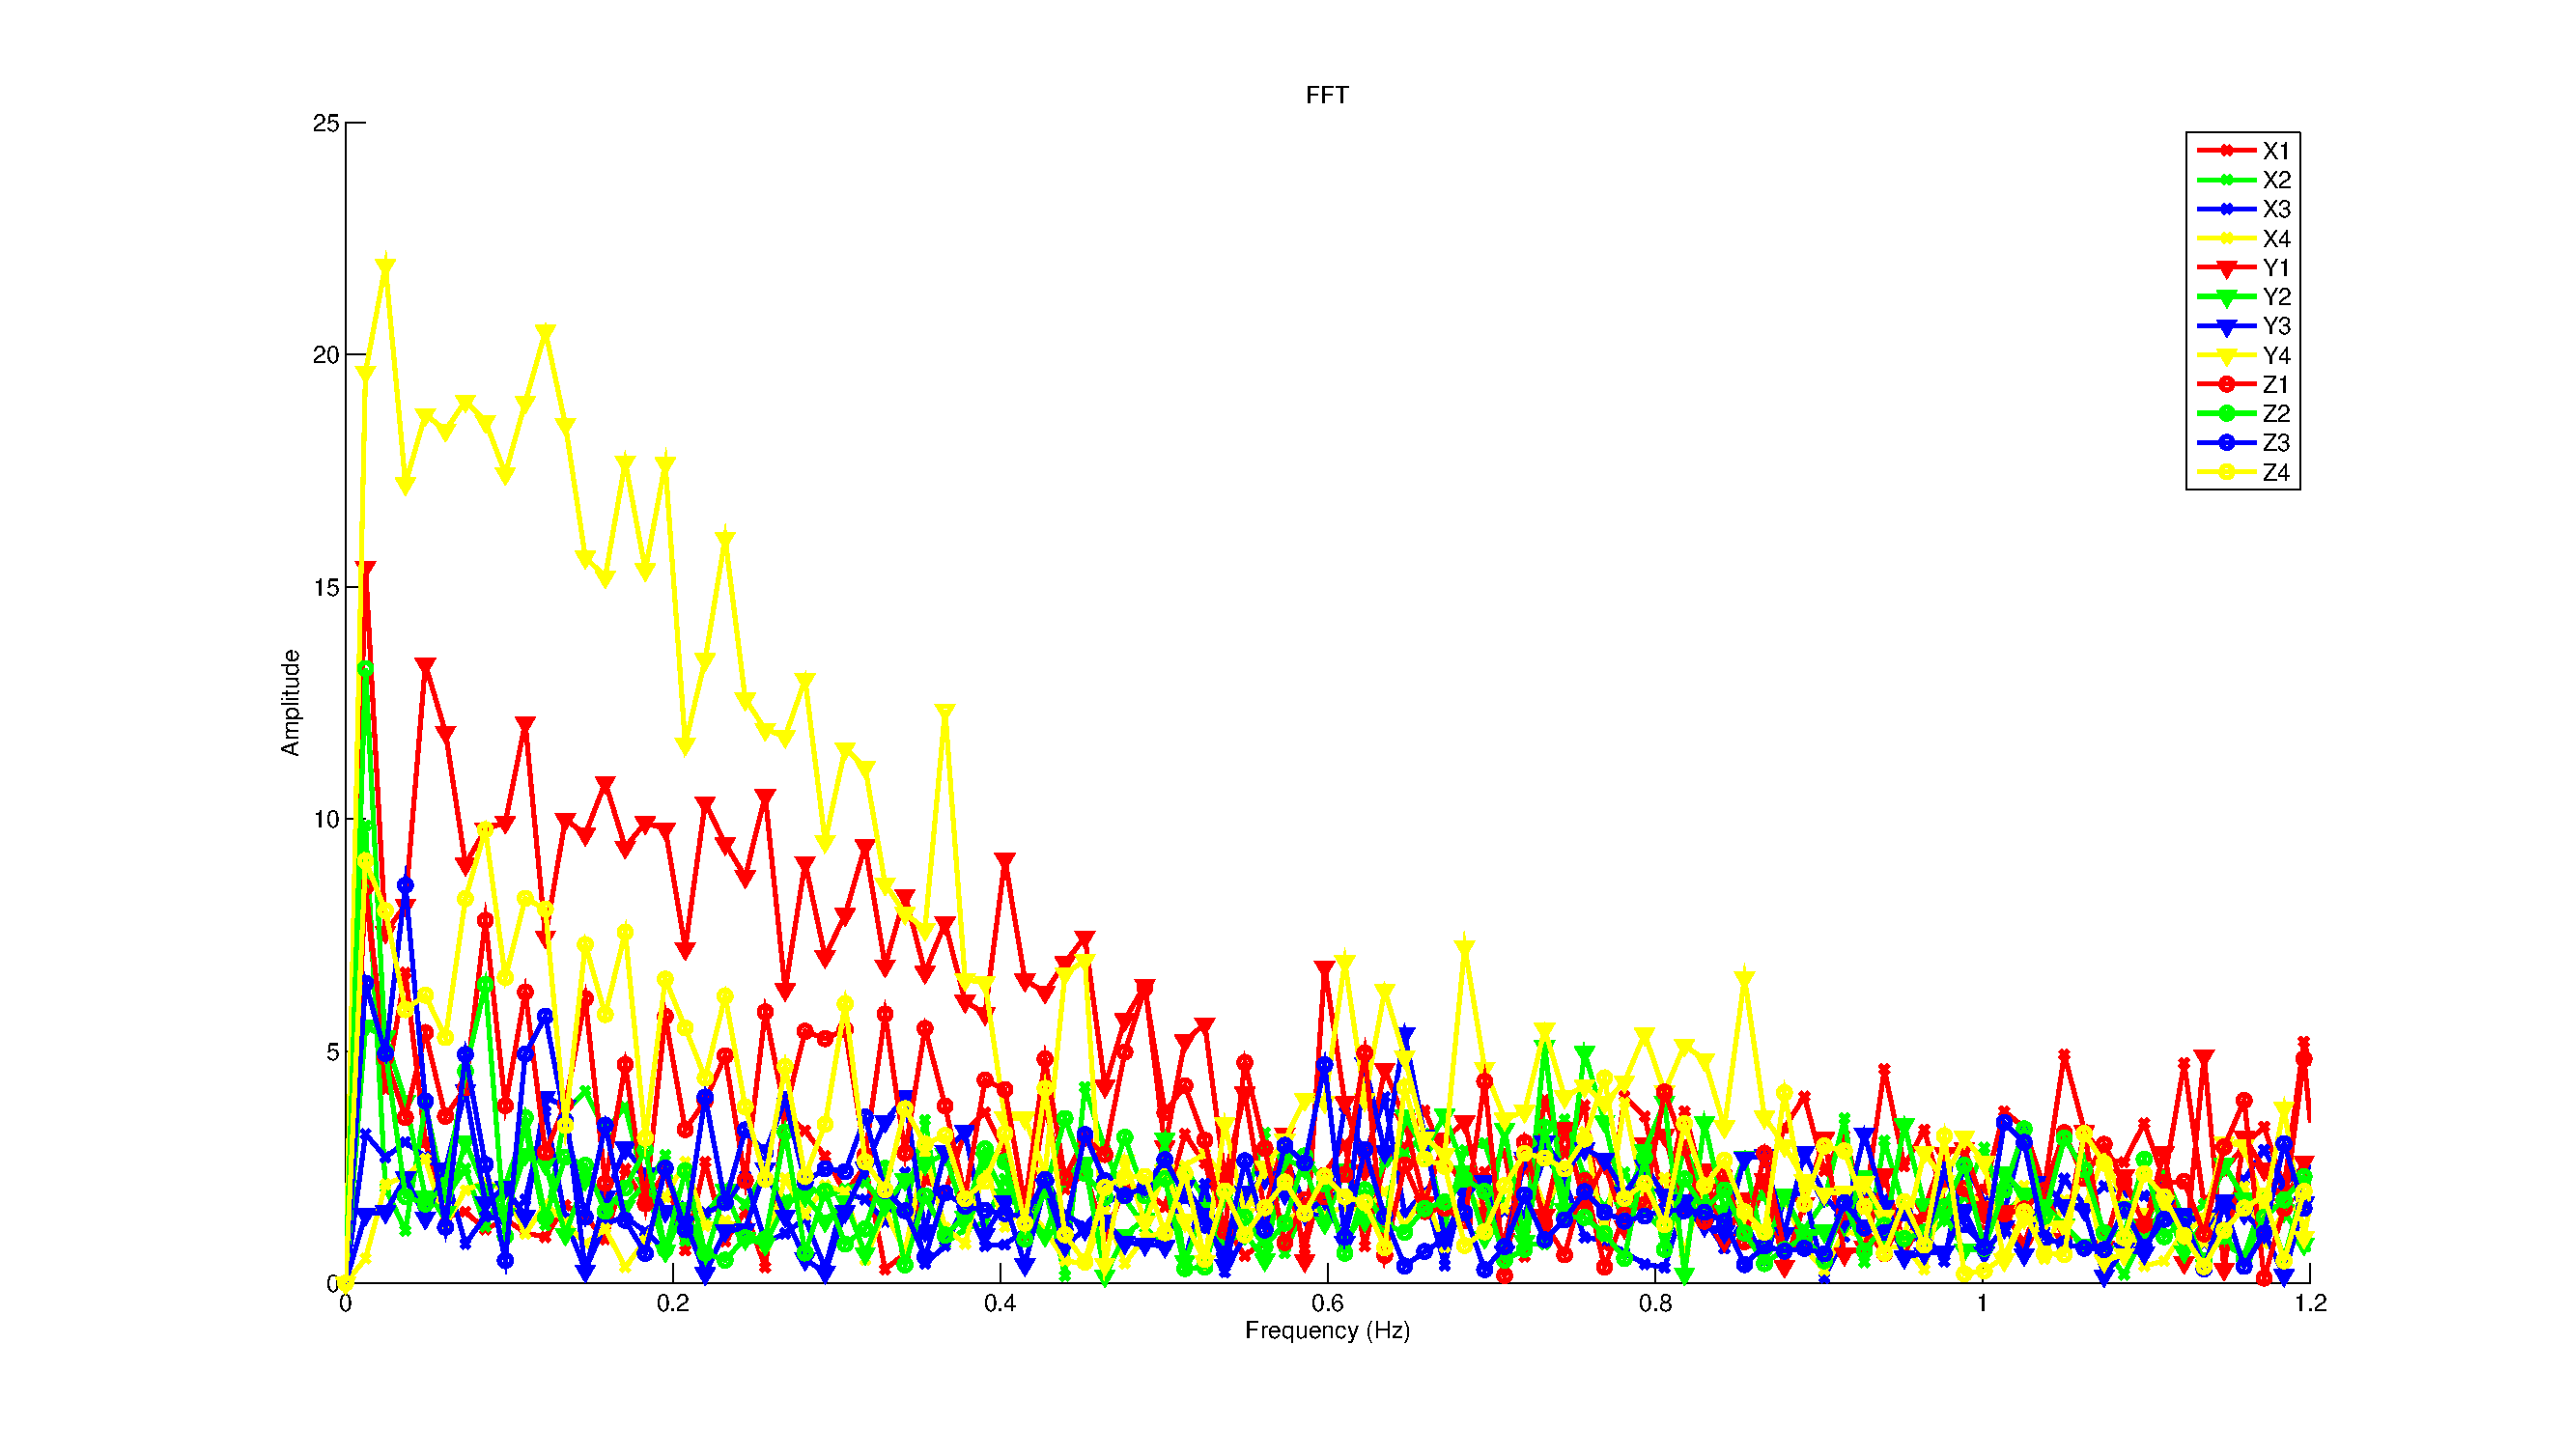
\includegraphics[width = \textwidth]{WESLEY_FFTallRAW.eps}
\caption{\textit{FFT of 6g data}}
\label{fig:fftall}
\end{figure}
